\documentclass[a4paper,twoside,11pt,openany]{book}
\usepackage[nomarginpar,margin=2.5cm]{geometry}
\usepackage{graphicx}
% \usepackage{showframe} % for testing
\usepackage{url}
\usepackage[binary-units,alsoload=hep]{siunitx}
\usepackage{natbib}
\usepackage{har2nat} % har2nat must be loaded after natbib.
\usepackage{bigstrut} % for row spacing in tables
\usepackage[version=3]{mhchem} % for chemical equations
\usepackage{GoudyIn,lettrine}
\renewcommand\LettrineFontHook{\GoudyInfamily}
\usepackage{verbatim} % for the comment environment
\newcommand{\URL}[1]{$\langle$\url{#1}$\rangle$}
\DeclareOldFontCommand{\bf}{\normalfont\bfseries}{\mathbf}
% This is the chapter titled `Optical TEMPEST' in Ireneusz Kubiak's new book.
\begin{document}
\title{New Book}
\author{Joe Loughry}
\setcounter{chapter}{6} % This chapter will be Chapter 7 of the book.
\setcounter{page}{263} % Page 263 will be the first page of this file.
\thispagestyle{empty}
\chapter{Optical TEMPEST}
\lettrine[lines=3]{T}{he} leakage of information out from a system through a
channel of modulated light is a vulnerability. The operative terms here are
`leakage',
`information', `channel', and `modulated light'. The \emph{leakage} might be
accidental or it may be caused on purpose by an adversary, but either way it
is not
supposed to be there. \emph{Information} can be anything from a single bit to
large volumes of information; it might be extremely small and high-value
information like
cryptographic keys. \emph{Channels}, in the Shannon sense \cite{Shannon1948}
have a bandwidth-delay product and noise; both of these are important to
understanding the risk of optical TEMPEST. And finally, \emph{modulated light}
carries the signal. Light can be modulated in time or in space---in this
chapter we think of
light modulated in the time domain. Light modulated in the space domain is an
\emph{image}; `shoulder surfing' is a real risk but not the one we are
concerned with here.\footnote{Shoulder surfing is the clandestine or covert
surveillance of display screens or keyboard activity for the purpose of
stealing secrets. It might be done visually or my means of a camera; it can
even be done without line-of-sight, by deconvolving a distorted reflection off
a shiny object in the optical path
\cite{Backes2008,Backes2009a,Raguram2011,Jenkins2013a,Xu2013a}. Optical
\emph{time-domain} eavesdropping on video displays \cite{Kuhn2002} is discussed
in \S \ref{section:Markus}.}

Further in the time domain, light can be amplitude-modulated,
frequency-modulated, phase-modulated, or polarisation-modulated. Amplitude
modulation (AM) is the only one that makes any kind of practicable sense for
optical TEMPEST purposes. The reason for this is because the modulation
capability, for anything other than amplitude modulation, simply is not there;
external hardware such as an electro-optic modulator is needed for those
methods. Amplitude modulation, on the other hand, is easy with the resources
available (and sometimes even happens accidentally). Optical TEMPEST
vulnerabilities most often depend on the accidental or improvised existence of
a modulated---or modulatable---channel, and AM is likely the simplest and most
straightforward modulation method to implement.

On-off keying (OOK) is the simplest AM method and the most likely to occur
accidentally, or to be achievable by an opportunistic adversary; in OOK, a
light being on means a binary 0 or 1, and light
off means the opposite. But OOK is not self-clocking: the receiver must
know {\it a priori}---or be able to discover---the sender's intended bit
interval to decode the signal; if the sender is able, there are better line
codes than OOK---Manchester coding, for example---that a deliberate sender
inside the target system may be able to use. But more often the adversary is
limited to exploiting sources and methods that are already there.

We shall discuss every aspect of optical TEMPEST in practice, from sources of
information and sources of radiation, through receivers, optics, and coding.
The number of conceivable vulnerabilities in this class is limited only by the
imagination of attackers, and even includes a few naturally occurring channels.
Follow along as we map out the landscape, beginning with the idea of
compromising emanations.
Figure \ref{figure:taxonomy} shows the taxonomy of optical TEMPEST in the
larger context of vulnerabilities due to \emph{compromising
emanations}---exploitable leakage of measurable physical phenomena out of a
system that can be interpreted by an adversary to gain information about the
internal state of the system (or, in some rare cases, to affect the internal
state of the target system). We shall now go through the taxonomy in detail.
\section{Compromising Emanations}
TEMPEST is concerned with the exploitation and control of compromising
emanations. These are unintended leakage of signals---interpreted here in the
widest possible sense, as anything at all that can be used by a clever
adversary---that carry information about what the target system is doing. Some
of the earliest research published about optical TEMPEST divided up the
vulnerability by the severity of the problem (Table \ref{table:class_III});
Class III optical emanations are what is usually known as an optical TEMPEST
vulnerability.

\begin{table}[ht]
\caption{The original classification system for risk level of optical TEMPEST
radiation. This table reproduced from \citeauthor{Loughry2002a},
\citeyear{Loughry2002a}.}
\medskip
\label{table:class_III}
\centering
\begin{tabular}{|l|l|c|}
\hline
\multicolumn{1}{|c|}{Type} & \multicolumn{1}{|c|}{Correlated to}
  & Associated Risk Level \bigstrut \\
\hline
\renewcommand{\arraystretch}{1}
Class I & State of the device & Low \\
Class II & Activity level of the device & Medium \\
Class III & Content (data) & High \\
\hline
\end{tabular}
\end{table}

Leakage from a system may be conducted or radiated; conducted emanations are
usually thought of as power supply vulnerabilities, but may also be conducted
through less obvious media, such as shared ground connections or structural
materials (even water pipes)
comprising a building. Radiated emanations include radio frequency (RF) or
shorter wavelength electromagnetic waves, up to and including light. TEMPEST
itself is
thought to be a code name for the suppression, masking, or control of RF (and
probably also acoustical)
compromising emanations; these are known to originate from---at least---cables
(communication or video), video displays (CRT or flat screen), and printers
\cite{NSAtempest2007,vanEck1985,Smulders1990,Kuhn2002,Grzesiak2010a}. Acoustic
vibrations---conducted or radiated---have been observed and successfully
exploited from keyboards, video displays, printers, and even computer
motherboards \cite{Wright1987,Asonov2004,Zhuang2005,Berger2006,Backes2010,
Genkin2013,Genkin2018a,Kubiak2018f}.

Mitigation of TEMPEST vulnerabilities, in the past when the risk was thought to
be limited to RF and acoustical emanations, was based largely on the idea of a
\emph{control zone}: to rely on the fact that emanations attenuate according to
an inverse square law---shield them as much as possible, but then employ fences
and guards to keep unauthorised receivers a safe distance away \cite[\S
17.4.2]{Anderson2008a}. The concept is a generalisation of the security
engineering principle of an `air gap' between systems handling classified
information. Recently, however, Clive Robinson has proposed a more general
concept of an `energy gap' that encompasses more than simply distance: in other
words, active and passive defences, cryptography work factor, and emanations
security extended throughout the electromagnetic, acoustic (or vibrational, or
seismic), and chemical spectra \cite{Robinson2018a,Robinson2018b}.

\begin{figure}[htp]
  \centering
  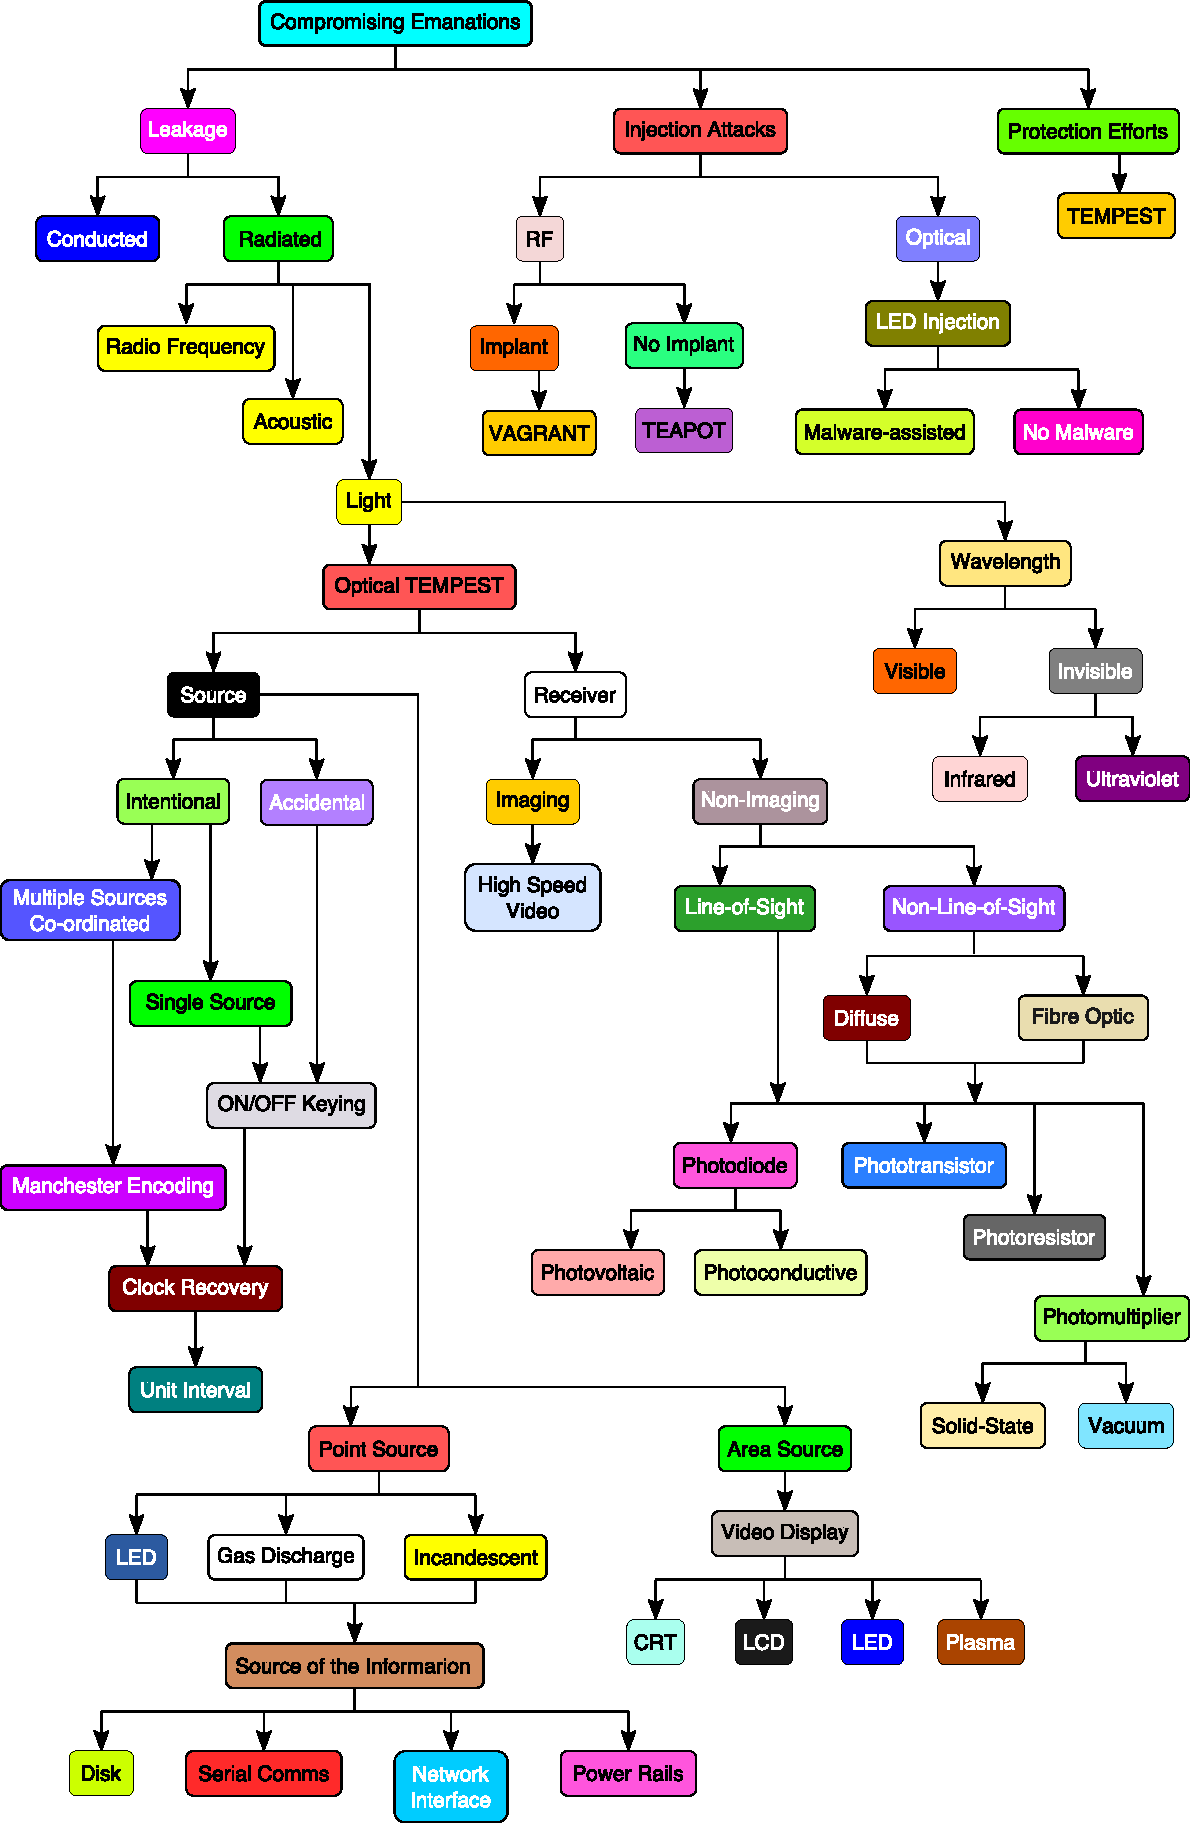
\includegraphics[width=\textwidth]{taxonomy.pdf}
  \caption{Taxonomy of optical TEMPEST in the larger context of compromising
    emanations.}
  \label{figure:taxonomy}
\end{figure}

\subsection{Light Sources}
Compromising emanations necessarily take one of two paths from source to
receiver: they may be conducted or
radiated. (Injection attacks are another matter and will be discussed in
\S \thechapter.\ref{section:injection_attacks}.) Optical emanations are always
of the radiated type; light is a species of electromagnetic radiation and
therefore follows an inverse square law---distance is the TEMPEST defender's
most valuable ally. Like with other electromagnetic radiation, wavelength
(colour) is important in optical TEMPEST. Wavelengths in the range of
approximately 350--\SI{700}{\nano\metre} are visible to
humans; wavelengths shorter than \SI{350}{\nano\metre} or longer than
\SI{700}{\nano\metre} are not. Visual indicators---such as light emitting
diodes, or LEDs---obviously must always radiate at visible wavelengths. But
invisible wavelengths cannot be completely discounted by optical TEMPEST
defenders because LED emitters at wavelengths outside the visual spectrum are
easily sourced. This brings up again the distinction between intentional and
accidental sources; accidental sources of optical emanations will almost always
be at visible wavelengths, whilst intentional sources may have the additional
flexibility to be able to employ invisible ones. This distinction can be useful
when forensically attributing intent.

Aside from wavelength, virtually the only other variable available to the
attacker is the coding method: simple or more complex.\footnote{In addition to
the advantage of invisible wavelengths, an attacker capable of arranging for
intentional optical emanations may also be able to specify a higher intensity
source than status indicators usually are.} Accidental sources are almost
always single sources and almost always employ OOK; an intentional attacker may
be able to co-ordinate multiple sources---either for improved reliability or
increased bandwidth---and may additionally have the flexibility to choose
self-clocking line codes such as Manchester encoding to simplify the clock
recovery problem. For accidental sources, or when an intentional source is
precluded from using self-clocking line codes, the problem of inferring the
unit interval and maintaining receiver synchronisation with the sender is
complicated. However, it is not impossible, as previously demonstrated
\cite[\S 8.2]{Loughry2002a}.

Light sources vulnerable to optical TEMPEST include visual indicators---a
subset of which are video displays---and discrete indicators. Indicators that
are controlled automatically are not as useful to an attacker as if they may be
set by the adversary. There are other sources to consider, however; infrared
(IR) illumination is one. Some smart light bulbs, such as the LIFX+ series,
contain an additional infrared (IR) emitter that is independently controllable
and has been employed as an invisible communication channel \cite{Maiti2018b}.

\subsection{Area Sources}\label{section:Markus}

Area sources include illumination and video displays. Video displays based on
cathode ray tube (CRT) technology used to be most prevalent but have largely
been replaced by flat-screen technologies including plasma, liquid crystal
displays (LCD), and light emitting diode (LED) arrays. From an optical TEMPEST
perspective, all have importantly different characteristics relating to speed.
CRT and plasma displays are both based on phosphor excitation; in the case of a
CRT, by a scanning electron beam, and for plasma displays, by a high voltage
glow discharge. In either case, the decay curve of the phosphor is what makes
an optical TEMPEST attack possible or not. Some phosphor formulations---those
typically used for radar displays---have a very slow decay; phosphors used in
video displays have a fast decay. What is needed for a successful optical
TEMPEST attack against a CRT or plasma display is a fast-decay phosphor, or one
with a `step' early in the decay curve, that is faster than the sweep of the
electron beam across one line of the video display. This is what
\citeauthor{Kuhn2002} (\citeyear{Kuhn2002} was able to exploit even though
earlier researchers had looked for such a signal and not found it. Plasma
displays, by their nature, need not be `swept' by a regular raster pattern as
are CRT displays, but oftentimes they are, for compatibility with existing
video signal transmission standards. It is the \emph{video} signal itself that
is exploitable, not individual pixels. This is important for understanding the
vulnerability of other two major flat screen display technologies: LCD and LED.

The most common display technology today is LCD. Both LCD and LED arrays need
not be raster-scanned the way CRT displays were; the newer technologies are
inherently pixel-oriented and could be directly addressed (as they often are in
very small devices, like pocket calculators) without the added complexity of
raster scanning. But for backwards-compatibility reasons, it is often more
cost-effective to add a raster-scanning interface layer that makes the new
display work like the old CRT displays, on a video signal. Interestingly,
\citeauthor{Kuhn2002} (\citeyear{Kuhn2002}) found that it was this extra
compatibility interface layer that was the source of most of the exploitable
TEMPEST radiation, in the RF region. If it wasn't the raster-scanning emulation
layer, then it was poorly-shielded cables between the computer and the display,
or inside the display, that were the richest source of RM emanations. This
tendency has continued to the present day.

\subsection{Point Sources}\label{section:incandescent}

Not counting video displays, point sources are by far the most common sort of
exploitable optical TEMPEST radiation sources. Incandescent lamps---which were
actually used for console indicators on early mainframe computers---make for
poor reception, as the filament has a relatively large thermal mass, imposing a
low-pass filter with a long time constant on the resulting blackbody radiator
(on the order of \SI{100}{\milli\second}). Gas discharge lamps, such as the
NE-2 neon glow lamp, are much faster, but not widely used these days.
Overwhelmingly, discrete indicators in the 21st century are LEDs.

\subsubsection{Optical Characteristics of Light Emitting Diodes}

LEDs are inexpensive, bright, require little power, and are available in many
different shapes and colours. All these qualities make them ideal visual
indicators. LEDs are also fast; {\it i.e.}, they turn on and off quickly, which
is less important, given the limitations of human eyes. (Turning LEDs on and
off more at more than about \SI{30}{\hertz} is pointless in most applications,
as a human will see only a steady glow.) The extra speed of LEDs is actually
used to advantage in persistence-of-vision (PoV) displays and pulse-width
modulation (PWM) dimming applications, which begin to hint at the possibilities
for high-capacity optical TEMPEST vulnerabilities.

To connect LED indicators to optical TEMPEST, consider the source of any
information impressed onto the visual indicator, as in Table
\ref{table:class_III}. Information may originate from storage device activity
(disk drives, tape drives, or emulated storage devices in memory), serial
communication channels---extremely common---or network interfaces. Serial comms
were actually where the first detectable optical TEMPEST emanations were found.

LEDs can be electrically modulated well into the \si{\mega\hertz} range by
standard digital logic circuits, even inadvertently. (As evidence, observe that
LEDs are used as fibre optic transmitters for---relatively---low speed links,
short distance links, up to a few \si{\mega\bit\per\second}.) In the case of
low-speed serial communications, up to a few \si{\kilo\bit\per\second}, the
visible flicker of a single LED tracking the mark/space state of a serial
communication channel is of benefit for routine monitoring and troubleshooting.

LED pilot lamp indicators on power rails are a surprising source of decodable
optical emanations, but perhaps less surprising in light of
\citeauthor{Kocher1999}'s (\citeyear{Kocher1999}) discovery of \emph{power
analysis}---the fact that carelessly implemented cryptographic algorithms,
running on commodity hardware, impose a time-varying load on the power supply
of the computer that can be measured and interpreted. Combined with finite
power supply regulation capacity and a good lock-in amplifier, secret keys can
be deduced one bit at a time. An LED directly connected to the power rail,
whilst intended as a simple power-on indicator, is fast enough, and sensitive
enough to microscopic changes in voltage, to effectively amplitude-modulate a
prefect mirror of the CPU's instantaneous power supply load as an optical
signal. Defences against this particular threat require interposing a low-pass
filter between the power rail and the LED, as described in \cite{Loughry2006a}.

\subsection{Channel Coding}

The source of optical emanations may be deliberate or accidental. The
accidental kind are more common. Accidental optical emanations may occur as a
result of hardware or software errors; hardware design errors are the usual
cause. Accidental optical emanations are modulated by accidental means, so very
simple channel coding is the most likely to be found: amplitude modulation
using on/off keying; the likelihood of more complex channel coding to occur by
chance is low, with the possible exception of some form of pulse width
modulation. Deliberate optical emanations have much greater latitude in form,
power, modulation, and coding.

Deliberate introduction of compromising optical emanations may be done through
any combination of hardware and/or software. Stimulated emanations by means of
software often make use of keyboard LEDs \cite[Appendix A]{Loughry2002a},
\cite{Zhou2018c}. The possibilities for an adversary
with access to make hardware modifications are vast: such an adversary might
employ multiple emitters, complex modulation schemes for speed, reliability, or
stealth; and even invisible wavelengths. It is demonstrably possible to
co-encapsulate multiple LED emitter chips (`dies') in a single standard
\SI{5}{\milli\metre} package, as evidenced by the availability of commercial
multi-colour LEDs. It is reasonable to assume, therefore, that a combination
visible/infrared LED might be produced, even without elaborate fabrication
facilities, so long as the epoxy envelope is transparent to both wavelengths.
Materials for such a chimera could be sourced commercially: dice from standard
LEDs---decapsulated in nitric acid (\ce{HNO3}) at about \SI{80}{\celsius}; wash
with acetone (\ce{(CH3)2CO})---with a lead frame salvaged from a standard
bi-colour LED,
de-soldered under a microscope, taking care to preserve the gold wire bonds,
then re-encapsulated in a low-viscosity UV-curing epoxy, chosen for
transmissivity at the desired wavelengths, in a silicone mould. The result
would be visually indistinguishable from a standard LED indicator except under
magnification, but would emit in both wavelengths at the same time.
Alternatively, a version could be made that emits visible light when
forward-biased and invisible light when reverse-biased, although that would
require more elaborate driver electronics. The greater efficiency of infrared
LEDs would mean that the luminous intensity at IR wavelengths would be much
higher than in the visible spectrum, thereby increasing the effective range of
the chimera LED.

Other possibilities open to the deliberate attacker with access to the hardware
design---either at the point of manufacture or intercepted later---include use
of multiple LED indicators simultaneously for one channel, either in parallel
(for more energy) or quadrature modulated (for reliability and ease of clock
recovery on the receiving end). Manchester coding, which is return-to-zero
waveform, has the advantage of being self-clocking, making the clock recovery
problem much easier. Use of several LEDs in a Manchester-like coding scheme
also has the advantage (for the transmitter) of modulating the LEDs at
approximately twice the data rate, likely making the visible flickering of the
LEDs less noticeable to an observer. This can be an advantage for stealth
\cite{Zhou2018c}.

\subsection{Sensors}
Given these sources of compromising emanations (accidental or intentional), to
have a communication channel there must be a receiver. Many kinds of optical
sensors will suffice, but what is needed particularly is an optical sensor with
a fast response time. Photodiodes, photomultipliers (solid state or otherwise),
phototransistors, photoresistors, or even some video cameras might be used.
Still cameras are not suitable, because this is a phenomenon integrated over
time.

There are two kinds of sensors: imaging and non-imaging. Imaging sensors have
some limited application in optical TEMPEST; they may be able to capture
multiple point
sources simultaneously, whilst co\"{o}rdinating those measurements in time,
which
can be useful in some situations, such as receiving from an entire rack of LED
indicators at once. But to do this, the imaging detector must have a very high
frame rate, and most video cameras do not. There exist high-speed video cameras
but there is usually a frame-rate--resolution trade-off, as well as a
frame-rate--sensitivity trade-off, so either (1) lines of resolution or (2)
light sensitivity, or both, must be sacrificed to gain a sufficiently high
frame rate. The minimum frame rate required is ideally at least twice the bit
interval of a serial data transmission, per Shannon's theorem.

Non-imaging detectors are more practicable. Non-imaging detectors may have a
direct line of sight to the source being observed, or not. If line-of-sight is
not possible, then of course the signal-to-noise ratio may be poor, but worse,
multiple sources, if they are active within the field of view of the detector,
may become intermingled. Optical signals at the same wavelength combine
additively. If that
happens, the situation is not in fact hopeless, as was demonstrated, at least
in simulation, in \cite[\S 8]{Loughry2002a}. There it was shown that multiple
uncorrelated sources, even having the same bit interval, could be separated
unambiguously despite the bit interval not being known {\it a priori}. As soon
as the line code can be determined with reasonable confidence, then the bit
interval can be guessed with high probability, and this is independent of the
individual bit intervals of $n$ uncorrelated signals. The time resolution of
the sensor, though, must be high, and low signal levels or a noisy detector
will make the problem more difficult.\footnote{As has been shown, however,
in numerous recent papers by other research groups, statistical recovery of
extremely low quality signals from acoustical vibrations, for example, is
highly amenable to machine learning (ML), hidden Markov models, and Fourier
analysis
\cite{,Asonov2004,Zhuang2005,Berger2006,Backes2010,Genkin2013,Kubiak2018f,
Genkin2018a}. Digital signal processing can pull a usable signal out of what
appears to be hopelessly noisy data; see \cite[Figure~4]{Loughry2002a}.} A
special case of non-line-of-sight \emph{imaging} interception
is the work of \citeauthor{Backes2008} \cite{Backes2008,Raguram2011,Xu2013a}.
these researchers showed that typed input and screen contents could both be
deconvolved from distorted reflections off shiny objects in the vicinity.
Another special case of non-line-of-sight optical TEMPEST is that of
fibre-optic media, either passively (eavesdropping via a dark fibre) or active
(observation of the un-capped radiation from a fibre-optic transmitter) but it
reduces to the same two problems as line-of-sight or non-line-of-sight optical
TEMPEST: as has been shown, if multiple signals at identical wavelengths are
additively mixed, they can be separated mathematically. (Optical filters or
spectroscopic methods can be used, if necessary, to separate overlapping
signals at different wavelengths. LEDs, however, are not very monochromatic, at
least compared with lasers.)

Optical detectors tend to be one of photoconductive, photoresistive, or
photoelectronic. Photoconductive detectors include photodiodes and
phototransistors; photodiodes generally are faster and more sensitive than
phototransistors, especially when operated in reverse-biased mode. Use of
photoresistors as optical TEMPEST detectors is rare, although there is one
recent example in the literature \cite{Barisani2009a}. The most sensitive
detectors---useful at long distances when the number of photons that can be
gathered from the target is low---are photomultipliers, either vacuum state or
solid state (avalanche photodiodes). One of the few vacuum state devices still
in use in 2019, photomultiplier tubes are superior in sensitivity, dynamic
range, and sometimes even response speed to photodiodes, and are ideal
detectors for optical TEMPEST. Their only drawbacks are cost, size, fragility,
and the requirement for special high voltage power supplies. Photomultiplier
tubes, however, have the advantage of not requiring a separate transimpedance
amplifier, which photodiodes do. Transimpedance amplifiers tend to have a severe
gain--bandwidth trade-off; at high gains (a few tens of \si{\deci\bel}), the
bandwidth may be only a few \si{\kilo\hertz}. In contrast, typical
photomultiplier tubes offer direct amplification of \SI{100}{\deci\bel}, and
when the optical flux is low, and the need for response speed high, a
photomultiplier tube cannot be beat.

Additional collection optics, {\it i.e.}, telescopes or fibre optics, are
useful for increasing the light-gathering capability of the detector; if light
levels from the source are low, external optics will improve the sensitivity of
the detector by the square of the aperture of the optics, divided by the area
of the detector (typically on the order of \SI{1}{\square\milli\metre}). While
the aperture of the collecting optics determines the amount of light collected,
the focal length of the eyepiece (if using a conventional telescope) determines
the field of view: $f/N$ numbers, for larger values of $N$, lead to a narrower
field of view, important when aiming. External optics can make all the
difference between a usable signal level and impossibly challenging conditions,
but pointing stability is crucial at high magnification to avoid vibrations.

\subsection{Covert Channels}
\label{section:injection_attacks}

Depending on the nature of the leakage, information leakage through optical
emanations may or may not be a covert channel. By the classical definition,
due to \cite{Lampson1973}, a covert channel is made from a pair of
communicating processes, but in many cases, the source of compromising optical
emanations is in hardware, not a programme running on the CPU.

\subsection{Injection Attacks}

A recently discovered new aspect of optical TEMPEST is injection attacks. In
the historical record of TEMPEST, the U.S.\ National Security Agency (NSA)
named TEMPEST, as far as we know. We don't even know for sure that the word is
not an acronym. TEMPEST is generally believed to be a code name,
\textsc{Tempest}. Evidence for it is shaky, but there was supposedly
another programme called \textsc{Teapot} that dealt with stimulated
compromising RF emanations \cite[p.~539]{Anderson2008a} and partially
corroborated in December 2013 by Edward Snowden (NSA ANT
Catalogue, 2013). The two names are suggestive of a connection through the phrase
`\textsc{Tempest} in a \textsc{Teapot}'---an American idiom---attributed at
least to Cicero (\emph{On the Laws}, 52 BC) \cite[p.~173]{Cicero2017}
but evidence in the open literature is scarce; the only clear original source
for the name is a single unclassified document dating from 1972 in which
everything related to emanations other than RF is redacted
\cite{NSAtempest2007}.

RF injection attacks have been known (or suspected) for a long time; the
discovery of a passive microwave RF eavesdropping device in the the U.S.\
embassy in Moscow in 1952 (seemingly in operation since 1945) was publicly
disclosed in 1960 \cite{Stong1968a}. It is thought to have been designed by
L\'{e}on Theremin. More recently, NSA's ANT catalogue lists several available
methods under the code name \textsc{Vagrant} for modulating a remotely
impressed carrier wave with, for example, the `red' signal of a VGA graphic
display by means of a chip embedded (by NSA) in the VGA cable connector's
shell.

The first report of the theoretical possibility of an \emph{optical} injection
attack came in 2018 at a conference in Amsterdam \cite{Loughry2018a}. The idea
stems from the discovery in 1973 by \citeauthor{Mims1973b} of the fact that
common LEDs are reversible: they can act as photodiode detectors, both in the 
the forward-biased (photovoltaic) and reverse-biased (photoconductive) modes
\cite{Mims1973b}.\footnote{Unintended photosensitivity of junction
semiconductor devices has been known since at least the nineteen-seventies;
UV-eraseable programmable read-only memory (EPROM) chips take advantage of the
fact.}

The phenomenon languished in obscurity for many years, used
occasionally by electronics designers for setting the brightness of a display
in sunlight, or for other low-cost sensing duties
\cite{MERL2003a,Karadaglic2007a}. But it wasn't until recently that the
confluence of several factors led to the possibility of an exploitable attack
vector. The first came in 1993, when ultra-high-brightness LEDs were invented
\cite{Stringfellow1997}. High brightness LEDs are capable of photovoltaically
generating significant amounts of power \cite{Allain2019}. The second advance
came in 1996, with the advent of general-purpose input/output (GPIO) pins with
programmable pull-up and pull-down resistors on commodity microcontrollers
\cite{Atmel2013}. GPIOs, provided in relative abundance by virtually all modern
microcontrollers, can be set under software control to be digital outputs
\emph{or} inputs. Programmable pull-up and pull-down resistors---intended for
use with switches and buttons or to allow subsystems to share a communication
bus like I\textsuperscript{2}C---are far more useful to an adversary because
they can be set in nonsensical ways.

This opens up the definite vulnerability that any attacker
with the capability to modify the software running on one of these
microcontrollers---ubiquitous in the Internet of Things (IoT)---can reverse the
operation of any convenient LED indicator and turn it into an optical receiver.

The following year, experimental results were presented at the same conference,
this time in Barcelona, Spain \cite{Loughry2019}. It was shown the attack is
possible in principle, under certain circumstances. In essence, the hardware
designer needs to have made a particular kind of mistake in the design, which
clears the way for the vulnerability.\footnote{The trick only works if the
designer chose to save a power pin by connecting an LED to a pair of GPIO pins,
which might make sense if unused GPIO pins happen to be available.} It is
absolutely a covert channel, because the attacker needs be able to control a
software process running inside the target system's security boundary. As such,
the vulnerability can be mitigated in two ways: firstly, by configuration
control of the embedded software; and secondly, by preferring certain
less-vulnerable circuit variants when designing in LED indicators. Note ({\it
cf.} \S\ref{section:incandescent}) that incandescent lamps used as visual
indicators are not vulnerable to this attack.

% I don't want to try to get permission to use these figures in a book.

\begin{comment}

\begin{figure}[ht]
  \centering
  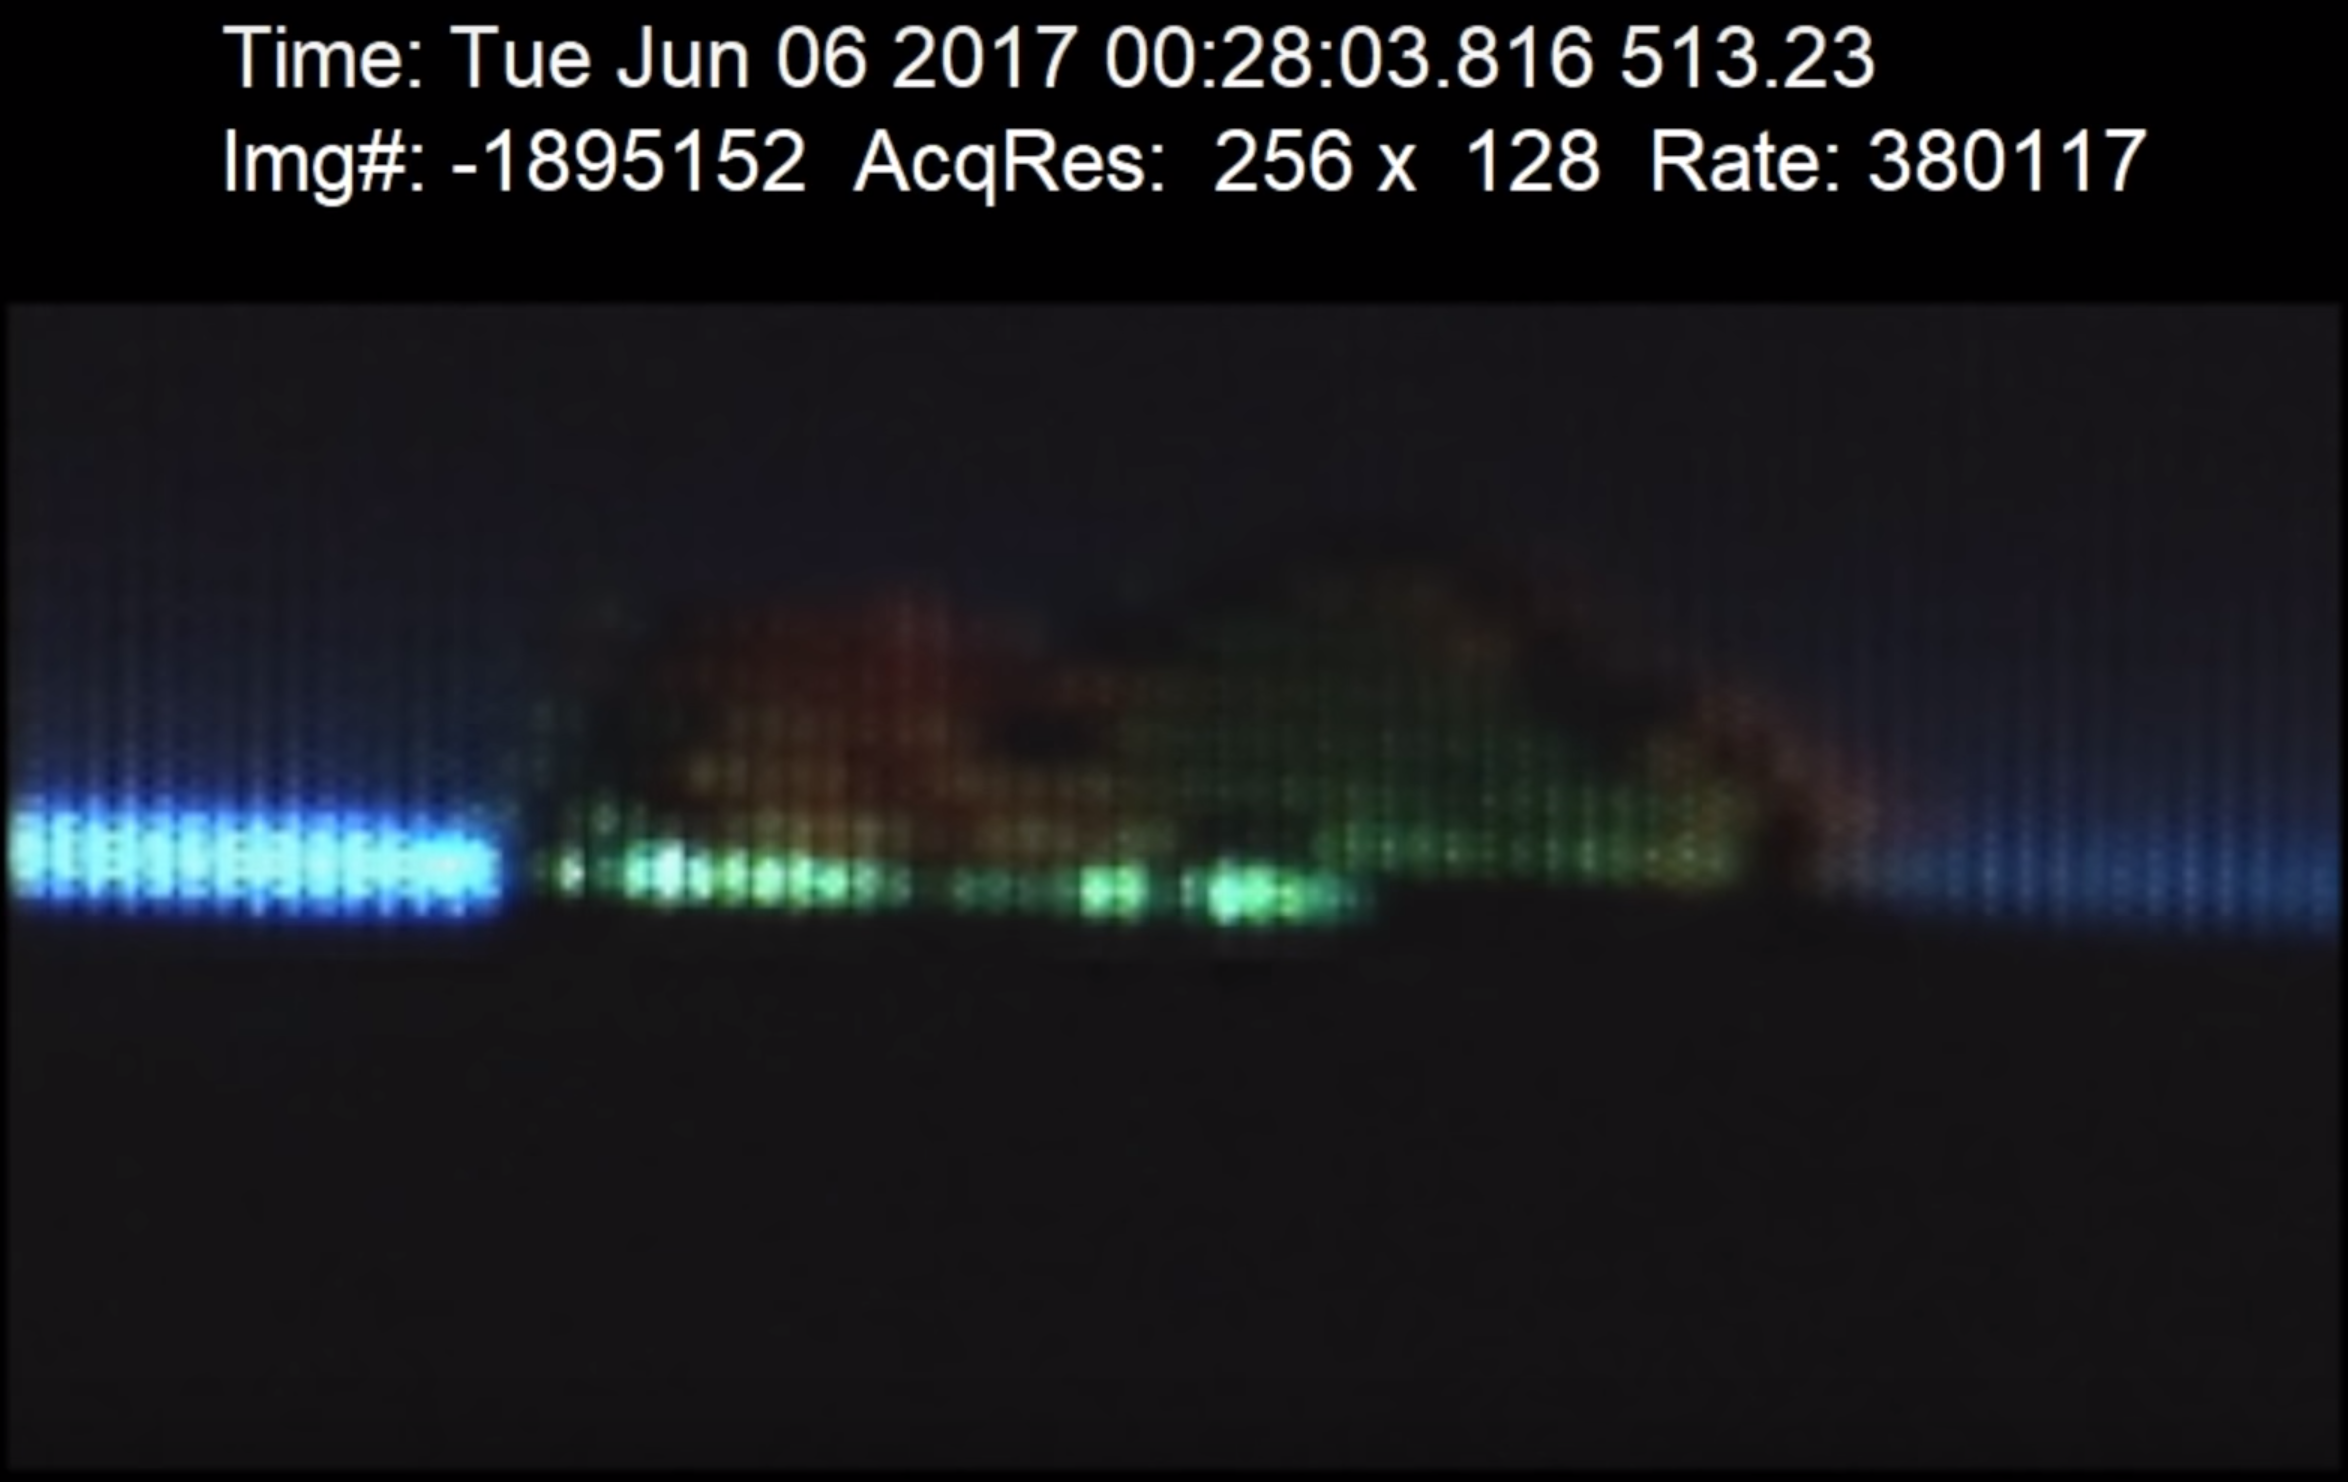
\includegraphics[width=3in]{slow-mo_guys_crt.png}
  \caption{High speed camera image (380\,117 frames per second) of CRT electron
    beam exciting phosphor dots \protect\cite{Free2018}.}
  \label{figure:slow-mo_guys_crt}
\end{figure}

\begin{figure}[ht]
  \centering
  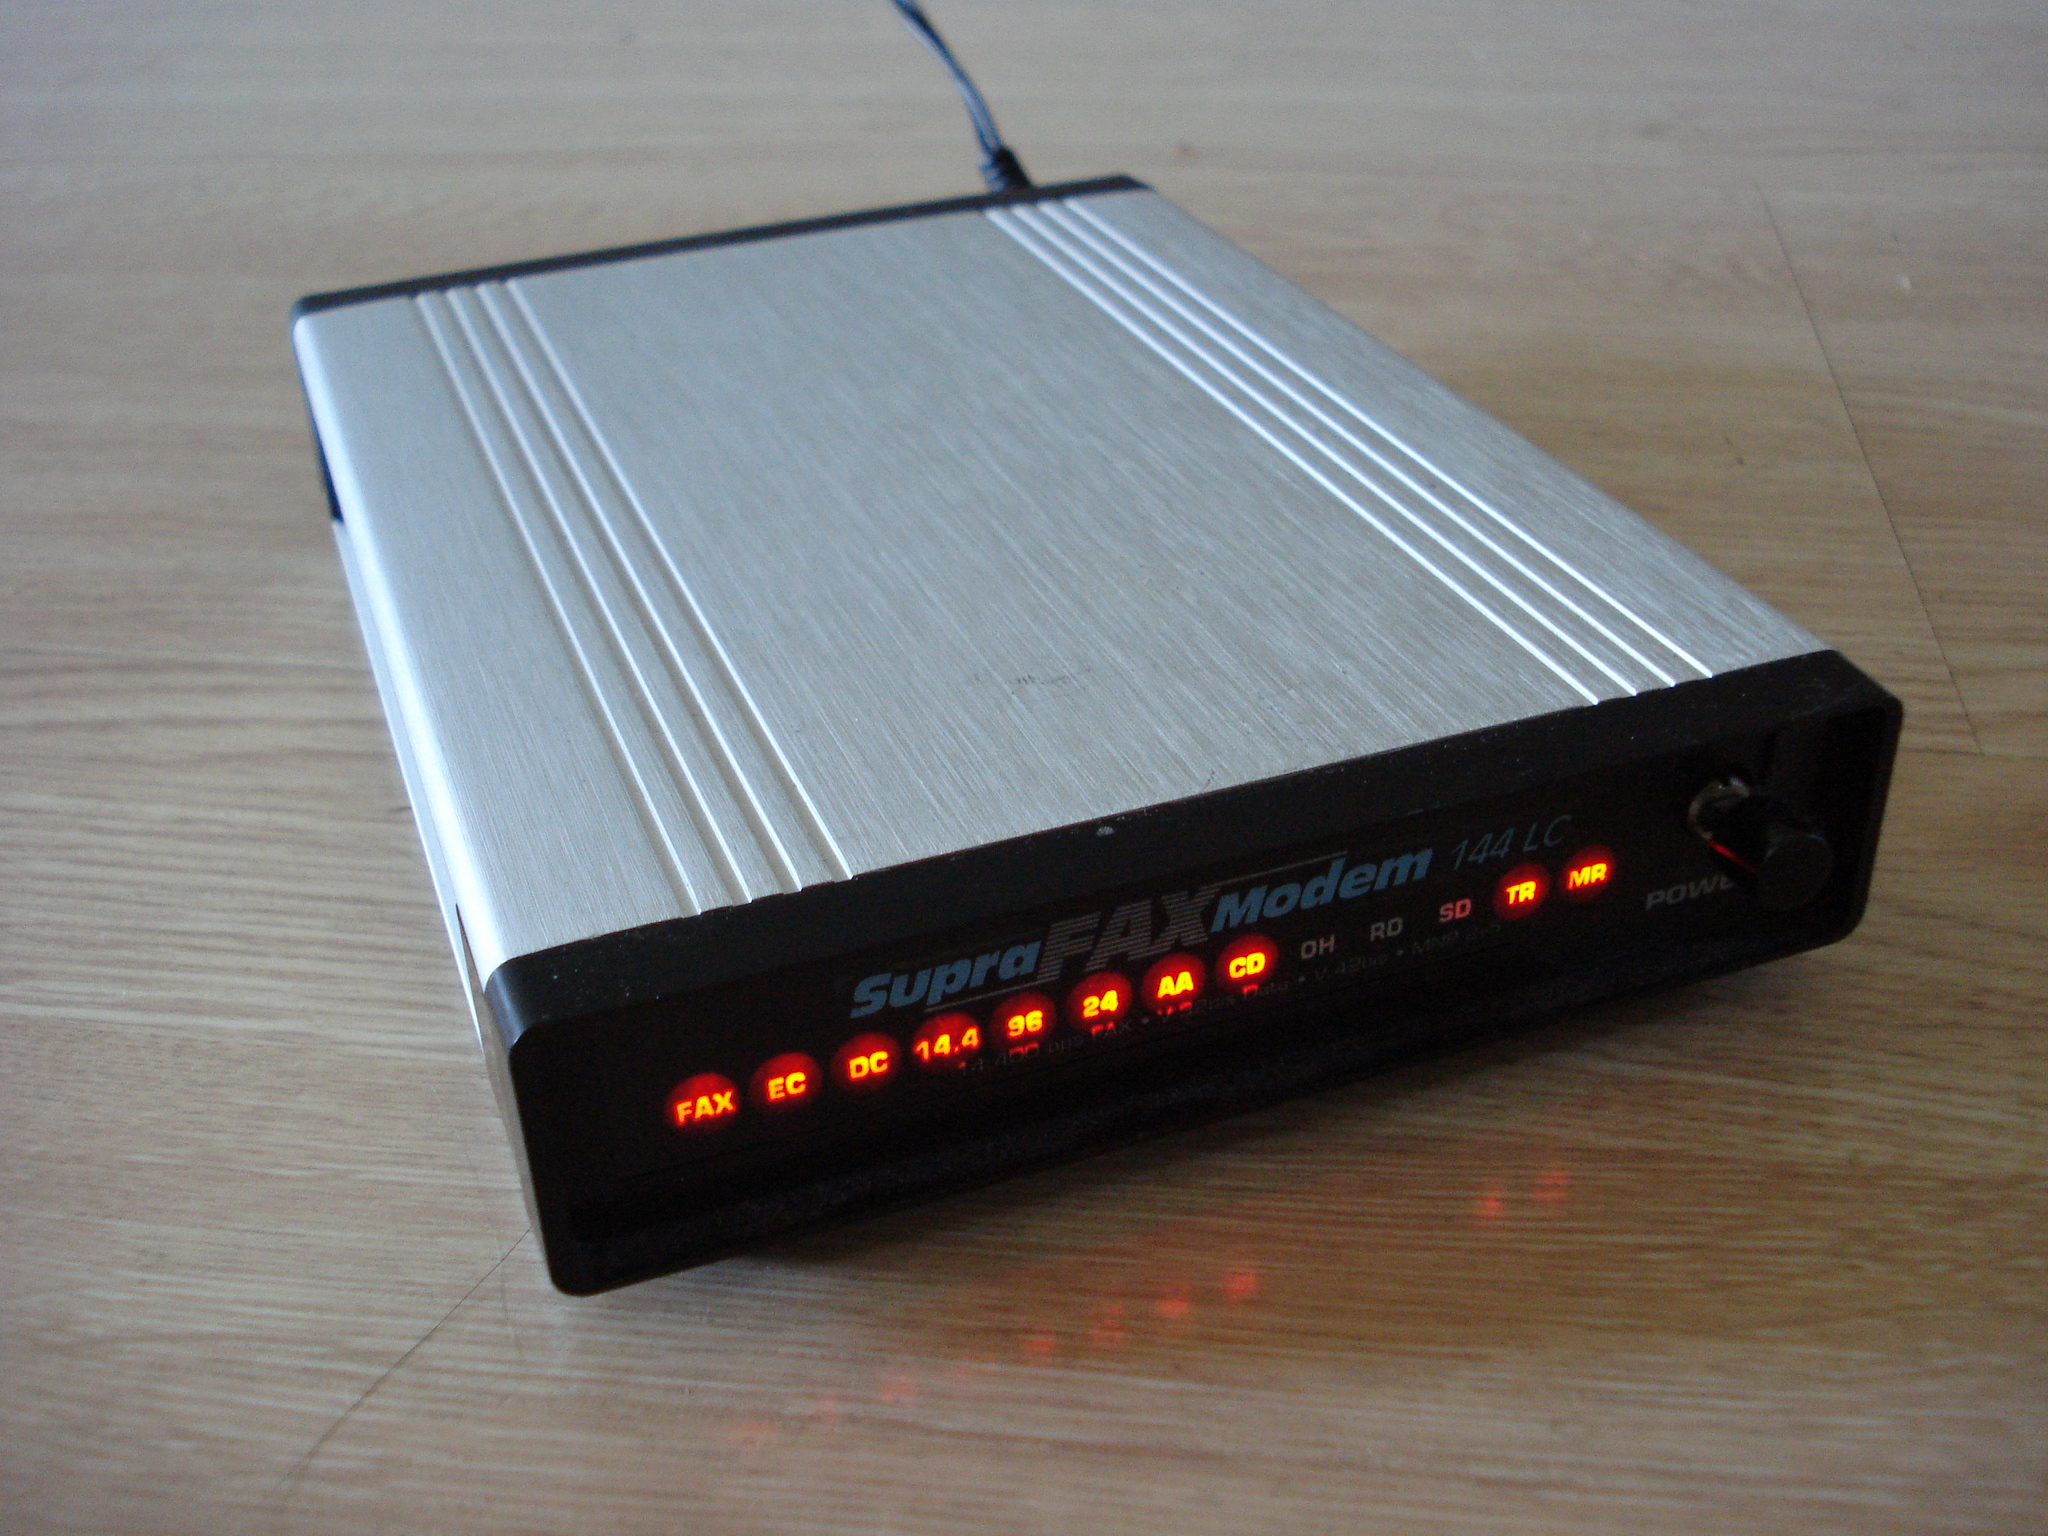
\includegraphics[width=3in]{SupraFAXmodem_144_LC_photo_courtesy_Wikipedia.jpg}
  \caption{Some LED indicators leak information.}
  \label{figure:modem}
\end{figure}

\end{comment}

\section{Conclusions}

The historical focus by TEMPEST military standard writers on RF and acoustic
emanations, and the fact that they overlooked optical methods (with the
exception of shoulder surfing) for so long, speaks to a sort of contextual
blindness. With the publication nearly two decades ago of the first two papers
about optical TEMPEST \cite{Loughry2002a,Kuhn2002}, open source information on
compromising emanations is booming. Before the year 2000, only a handful of
articles had been published in the unclassified literature on the subject of
TEMPEST or emanations security. The most famous was \citeauthor{vanEck1985}
(\citeyear{vanEck1985}), squarely in the traditional domain of RF.
(Interestingly, few books mentioned acoustic emanations; the concept was nearly
lost until rediscovered by the academic community in the early 2000s.) Covert
channel analysis, following the publication of the Rainbow series in
\citeyear{NCSC-TG-030}, similarly died out, probably from existential despair
\cite{NCSC-TG-030}. \citeauthor{Kocher1999}'s seminal paper on side channels
reignited interest in what \cite{Wright1987} had been saying for decades, and
since then, the spectrum has been widened to include magnetic fields and
gravitational waves \cite{Guri2018b,Abbott2016b}.

\bibliographystyle{./agsmitalic} % This is my twiddled version of agsm.bst.
\bibliography{consolidated_bibtex_file}
\end{document}
